\chapter{Curvature}

Given a connection on a fibre bundle, values in the bulk may be parallel transported along a curve in the base manifold.
If the curve is a closed loop, then values are not necessarily mapped back onto themselves.
The action of parallel transport around a loop known as its \textdef{holonomy}, and its failure to be the identity operator is a measure of the connection's \emph{curvature}.

Curvature may be restated as the obstruction to the \emph{integrability} of the connection.
Therefore, the curvature of a connection may be derived by finding the integrability condition of the parallel transport equations, which is most easily done via Frobenius' theorem.
\todo{Cite.}

\section{Integrability and Frobenius' Theorem}
\label{sec:Frobenius}

A connection $H$ is integrable if there exist maximal integral manifolds $f ∈ \secs(ℱ)$ such that $∇ f = 0$ everywhere, in which case parallel transport is path-independent, and loop holonomy is always trivial.

Suppose $\fibrebundle V 𝒱 ℳ$ is a vector bundle with a linear connection $∇$.
Elaborating the condition $∇ f = 0$, we have
\begin{align}
	\label{eqn:covariantly-const}
	∇_𝒖 X = 𝒖(X) + Γ(𝒖)X = 0
	\qqtext{or}
	∂_μ X^a = -Γ_μ{}^a{}_b X^b
\end{align}
everywhere for all $𝒖 ∈ \TT ℳ$.
As an Ehresmann connection, $H$ is the tangent subbundle described by these equations.

To express this, introduce coordinates $\set{x^μ}$ of $ℳ$ and linear coordinates $\set{x^a}$ of $V$ with respect to some basis.
A point $X ∈ 𝒱$ is a base point $π(X) ≡ (X^μ) ∈ ℳ$ together with a fibre value $(X^a) ∈ V$, having total coordinates
\begin{math}
	X = (X^μ, X^a)
.\end{math}
Similarly, a vector in $\TT_X 𝒱$ has components
\begin{math}
	δX = (δX^μ, δX^a)
.\end{math}

Such a vector $δX ∈ \TT_X 𝒱$ satisfies \cref{eqn:covariantly-const} if $δX^a/δX^μ = -Γ_μ{}^a{}_b X^b$, and hence the Ehresmann connection may be given by
\begin{align}
	H_X = \spanof{(δX^μ, -Γ_μ{}^a{}_b X^b δX^μ) | (δX^μ) ∈ \TT_Xℳ}
\end{align}
for each $X ∈ 𝒱$.
Geometrically, this describes the change in vector components $δX^a$ induced by a nudge in the base point $δX^μ$ if $X$ is constrained to move along $H$.

While it is always possible to take a point $X ∈ 𝒱$ and parallel transport it to form a $1$-dimensional integral curve of a tangent subbundle, it is not always possible to obtain higher-dimensional integral surfaces.
The existence of maximal integral surfaces requires a special property known as \emph{involutivity}.
\begin{definition}
	A tangent subbundle $𝒟$ is \textdef{involutive} if $[𝒟, 𝒟] ⊆ 𝒟$.
	That is, if for any two sections $𝒖, 𝒗 ∈ \secs(𝒟)$ in the subbundle, their Lie bracket $[𝒖, 𝒗] ∈ \secs(𝒟)$ also lies in the subbundle.
\end{definition}
The importance of involutivity is the content of Frobenius' theorem.
\begin{theorem}[Frobenius’]
	If $𝒟$ is a tangent subbundle, then
	\begin{align}
		\text{$𝒟$ is integrable}
		\quad ⟺ \quad
		\text{$𝒟$ is involutive}
	.\end{align}
\end{theorem}
Frobenius’ theorem can be dualised into a statement about exterior differential systems instead of vector subbundles, which can be more useful for calculation.
This stems from the observation that a vector subspace $U ⊆ V$ may be represented by the subspace $Ω$ of $1$-forms with $U$ in their kernels,
\begin{align}
	Ω = \set{ω ∈ V^* | ω(𝒖) = 0, \forall 𝒖 ∈ U} ⊆ V^*
.\end{align}
The original subspace $U$ is recovered as $U = \bigcap_{ω ∈ Ω} \ker ω$.

\begin{definition}
	The ideal $I$ associated to a tangent subbundle $𝒟$ is the ideal\sidenote{
		Recall from \cref{def:ideal} that an ideal (of forms) is closed under addition and satisfies $α ∧ ω ∈ I$ whenever $ω ∈ I$, for \emph{any} $α$.
	} generated by the $1$-form annihilators of $𝒟$,
	\begin{align}
		I = \gen{ω ∈ \forms[1](ℳ) | ω(𝒖) = 0, \forall 𝒖 ∈ \secs(𝒟)}
	.\end{align}
\end{definition}


The following lemma shows how the condition that $ℐ$ is an integral manifold translates between tangent subbundles and ideals.
\begin{lemma}
	Let $𝒟$ be a tangent subbundle and $I$ is its associated ideal.
	Suppose $ℐ$ is a submanifold with the inclusion map $ι : ℐ → ℳ$.
	Then,
	\begin{align}
		\text{$ℐ$ is an integral manifold}
		\quad ⟺ \quad
		𝒟|_p = \TT_pℐ
		\quad ⟺ \quad
		ι^*I = 0
	.\end{align}
\end{lemma}
\begin{proof}
	The first equivalence is by definition (but is included for readability).
	For the second equivalence, assume $ℐ$ is an integral manifold.
	Then, if $𝒖 ∈ \TT ℐ$ then the inclusion $\dd ι(𝒖) ∈ 𝒟$ lies in the tangent subbundle.
	Suppose $ω ∈ I$ so that $ω(𝒗) = 0$ for all $𝒗 ∈ 𝒟$.
	The restriction of $ω$ to $ℐ$ via the pullback $ι^*ω$ is identically zero, because
	\begin{align}
		(ι^*ω)(𝒖) ≡ ω\qty(\dd ι(𝒖)) = 0
	.\end{align}
	Since $𝒖$ and $ω ∈ I$ are arbitrary, we write $ι^*I = 0$.
\end{proof}



\begin{marginfigure}
	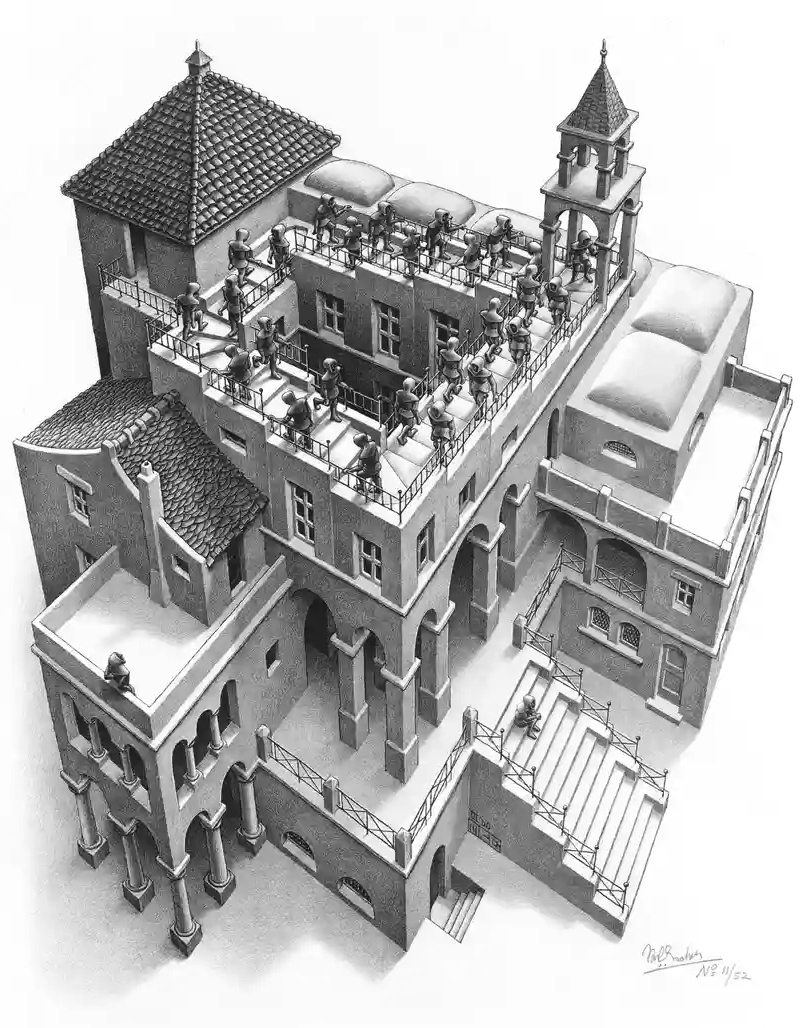
\includegraphics[width=1.05\columnwidth]{figures/penrose-stairs.png}
	\caption{
		\emph{``Ascending and Descending'' by M.\ C.\ Escher, 1960} --- perhaps the most famous illustration of an inexact $2$-form (the slope of the stairs) and its inconsistent `integral' (the impossible staircase).
	}
\end{marginfigure}
\begin{theorem}
	\label{thm:frobenius}
	If $𝒟 ⊆ \TTℳ$ is a tangent subbundle and $I ⊆ \forms[1](ℳ)$ is its associated ideal, then
	\begin{align}
		\text{$𝒟$ is involutive}
		\quad ⟺ \quad
		\dd I ⊆ I
	.\end{align}
\end{theorem}
\begin{proof}
	The ideal $I$ is generated by $1$-forms $ω$ which vanish when evaluated in $𝒟$, i.e., $ω(𝒖) = 0$ for all $𝒖 ∈ \secs{𝒟}$.
	If $𝒖, 𝒗 ∈ \secs(𝒟)$ then
	\begin{align}
		\label{eqn:xd-lb-identity}
		\dd ω(𝒖, 𝒗) &= 𝒖\qty(ω(𝒗)) - 𝒗\qty(ω(𝒖)) - ω([𝒖, 𝒗])
	\\	&= - ω([𝒖, 𝒗])
	,\end{align}
	since $ω(𝒖) = ω(𝒗) = 0$.
	If $𝒟$ is involutive then $[𝒖, 𝒗] ∈ \secs(𝒟)$ and $\dd ω(𝒖, 𝒗) = 0$.
	Thus, $\dd ω ∈ I$ if and only if $𝒟$ is involutive.
\end{proof}

Stokes’ theorem states that a differential form $φ$ is integrable if it is exact (i.e., if $φ = \dd ϕ$).
On a contractible domain, this is equivalent to $φ$ being closed, by Poincaré's lemma.
In the same vein, \cref{thm:frobenius} states that an exterior differential system is integrable over a contractible domain if and only if its associated ideal is closed.


\subsection{Curvature as an obstruction to integrability}
